
\chapter{Marco te\'orico}
\label{sec:chapter3}

\section{Aprendizaje M\'aquina}

Como se menciona en \cite{9780471056690} ``En el sentido m\'as amplio,
 cualquier m\'etodo que incorpore informaci\'on de ejemplo para el 
 entrenamiento en el dise\~no de un clasificador emplea aprendizaje''.
 Lo cual es evidente en el aprendizaje supervisado ya que en este existe 
 un maestro expl\'icito que proporciona la informaci\'on etiquetada
 \cite{9780471056690}, para que sirva de ejemplo al algoritmo de los casos 
 desconocidos que se le presentaran m\'as adelante. Pero en el aprendizaje 
 no supervisado, no requiere un maestro expl\'icito \cite{9780471056690}, sin 
 embargo, se le proporciona informaci\'on sobre la tarea, por ejemplo, el 
 n\'umero de grupos en los que hay que separar la informaci\'on proporcionada.


En los textos \cite{9780471056690, 9780387310732} se menciona el aprendizaje 
 por refuerzo (RL, por sus siglas en ingl\'es) como otra divisi\'on, ya que 
 a est\'e se le proporciona un conjunto de pol\'iticas de recompensa para 
 cumplir con un objetivo espec\'ifico, en lugar de ejemplos etiquetados como 
 en el caso del aprendizaje supervisado, estas reglas indicaran de forma 
 binaria cuales acciones le permite maximizar la recompensa por prueba y error.


El aprendizaje por demostraci\'on (LfD, por sus siglas en ingl\'es)
 \cite{ARGALL2009469} es una metodolog\'ia de aprendizaje m\'aquina, que a 
 partir del ejemplo de la tarea objetivo (proporcionado por un maestro o
 experto) se generan las pol\'iticas necesarias, para que por medio del 
 aprendizaje por refuerzo, el aprendiz realice la tarea.


Una de las principales caracter\'isticas de esta \'ultima metodolog\'ia
 mencionada, es la forma de adquisici\'on de datos; tele-operaci\'on o 
 sombreado. Para la tele-operaci\'on\cite{ARGALL2009469}, el aprendiz va 
 a grabar desde sus propios sensores mientras que el maestro va a manipularlo 
 desde un controlador o con sus propias manos, esto proporciona 
 un mapeo directo entre la acci\'on grabada y la acci\'on a realizar. Por 
 otro lado, el sombreado\cite{ARGALL2009469} requiere un algoritmo adicional 
 de mapeo, ya que est\'e seguir\'a las acciones realizadas por el maestro por 
 medios visuales y marcadores en el maestro, mientras graba de sus propios 
 sensores. 


La forma de procesar los datos recabados en la adquisici\'on de datos para 
 obtener las pol\'iticas de recompensa para el RL puede ser por: funci\'on 
 de mapeo, plan o modelo del sistema. El usar una funci\'on de mapeo 
 \cite{ARGALL2009469} puede ser en un enfoque continuo (Regresi\'on) o 
 discreto (Clasificadores); los algoritmos de regresi\'on pueden ser a modo 
 de ejemplo, aprendizaje lento (lazy learning, en ingl\'es) o regresi\'on 
 ponderada localmente (locally weighted regression, en ingl\'es); los 
 clasificadores usados para para el enfoque discreto pueden ser KNN 
 (k-Nearest Neighbors, en ingl\'es), \'arboles de decisi\'on, redes
 neuronales, etc.
 

Para obtener las reglas a trav\'es de un modelo de sistema\cite{ARGALL2009469}
 se realiza un mapeo del mundo en el que se va a desenvolver el aut\'omata 
 y a partir de este con los datos recabados se generan las pol\'iticas de 
 recompensa. Mientras que para usar un plan\cite{ARGALL2009469}, solo se 
 considera la secuencia de acciones desde un estado inicial a un estado final 
 objetivo con estados condicionales previos y resultantes. 

\section{Tipos de programaci\'on}

Para programaci\'on orientada a objetos (POO) se tiene la siguiente
 definici\'on:


``La programaci\'on orientada a objetos es un m\'etodo de implementaci\'on
 en el que los programas se organizan como colecciones de objetos cooperativos,
 donde cada uno representa una instancia de alguna clase y \'estas clases 
 son todas miembros de una jerarqu\'ia de clases unidas por herencia'' 
 \cite{020189551X}.


Algunas de las ventajas de la POO sobre la programaci\'on procedimental
 son la modularidad y la reutilizaci\'on de c\'odigo, facilitando el 
 desarrollo de programas, como si solo se unieran ``bloques de construcci\'on'' 
 \cite{020189551X}, tambi\'en, existe el encapsulamiento de los datos, lo 
 cual permite controlar el acceso a la informaci\'on almacenada 
 \cite{8448132467}. Adem\'as, el tipo de abstracci\'on es diferente en 
 un lenguaje procedimental a uno que es orientado a objetos, 
 ya que se trata de modelar objetos del mundo real en el programa y en 
 lugar de empezar por la definici\'on de las estructuras de datos y 
 procedimientos a usar, se empieza el desarrollo pensando en el objeto y 
 cuales son las tareas a desempe\~nar de ese objeto, lo que facilita la 
 implementaci\'on de una idea \cite{8448132467}. 


``En un lenguaje orientado a objetos verdadero, toda entidad en el dominio
 del problema se expresa a trav\'es del concepto de objetos'' 
 \cite{8448132467}, entre los lenguajes orientados a objetos Python
 \cite{MarzalVar2014} y \texttt{C\#} \cite{8448132467}, mientras que
 \texttt{C++} \cite{8448132467} no es un lenguaje orientados a objetos y 
 ``\ldots java, tan bueno como es, tiene algunas limitantes como lenguaje 
 orientado a objetos'' \cite{8448132467}.


``Se dice que un sistema de software est\'a basado en eventos si sus partes
 interact\'uan principalmente usando notificaciones de eventos'' 
 \cite{9781430201564}. Los sistemas Operativos con interfaz gr\'afica est\'an 
 basados en eventos, ya que la interfaz grafica de usuario (GUI, por sus siglas en 
 ingl\'es) espera de forma pasiva a que el usuario realice alguna acci\'on sobre 
 los controles \cite{9781430201564} (botones, cuadros de texto, etc). La 
 programaci\'on basada en eventos empez\'o a tener su relevancia a principios de 
 los a\~nos 90 con el surgimiento de Microsoft Visual Basic \cite{9781430201564}.
 
  
Considerando que el paso de mensajes entre las diferentes partes de un sistema
 para poder sincronizar \'estas \cite{9781430201564} es una caracter\'istica que 
 distingue a este paradigma de la programaci\'on, aquel lenguaje de programaci\'on 
 que permita el uso de hilos y sus m\'etodos de sincronizaci\'on, se puede decir 
 que permite la programaci\'on basada en eventos, esto sin mencionar los que son 
 compatibles con alg\'un framework para desarrollar GUI similares y/o compatibles
 con Microsoft Windows.



\section{Grafos}
Un grafo consiste en dos conjuntos finitos: un conjunto no vac\'io de
 v\'ertices y un conjunto de aristas, donde cada arista esta asociada 
 a uno o dos v\'ertices llamados puntos extremos\cite{SUSANNAS.EPP2012}. 
 Se dice que una arista incide sobre cada uno de sus puntos extremos, 
 dos aristas que inciden en el mismo punto se llaman adyacentes y el 
 v\'ertice en el que no incide ninguna arista se llama 
 aislado\cite{SUSANNAS.EPP2012}, En la figura \ref{fig:igrafo} se
 presenta un grafo que muestra las acciones dosponibles con el 
 teclado y rat\'on.
 
\begin{figure}[h]
\centering
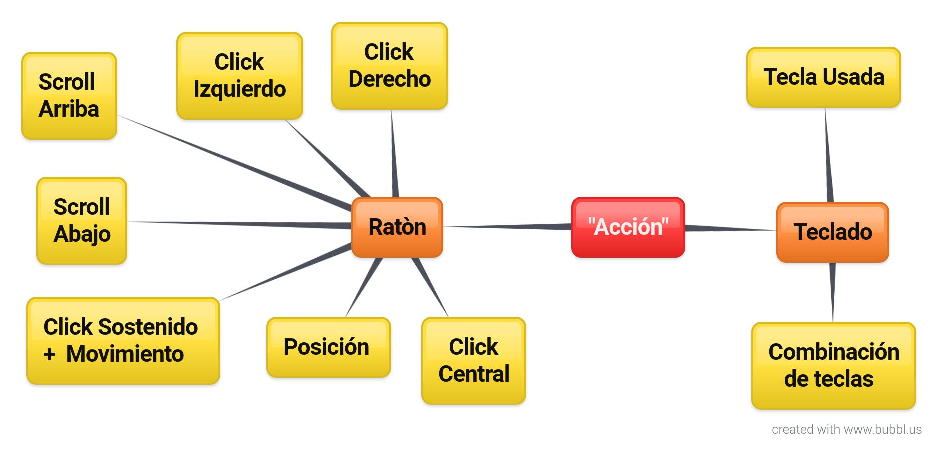
\includegraphics[width=0.8\columnwidth]{chap3/Imagenes/Grafo.eps}
\caption{Ejemplo de un grafo.}
\label{fig:igrafo}
\end{figure}


\subsection{Grafo Dirigido}
Un grafo dirigido se define por ser un grafo donde cada arista es un 
 par ordenado asignando la direcci\'on del primer elemento mencionado 
 al segundo\cite{SUSANNAS.EPP2012}. \'este tipo de grafo se puede 
 representar, en t\'erminos de programaci\'on,  como una lista enlazada, 
 la cual es ``una colecci\'on lineal de objetos de una clase autoreferenciada, 
 conocidos como nodos'' \cite{deitel2008java}, a \'estas solo se les puede 
 referenciar por el primer nodo, sin embargo, como cada elemento tiene la 
 referencia al siguiente se puede acceder a todos los elementos de la lista, 
 la ventaja ofrecida es la posibilidad de crear una lista de dimensi\'on 
 variable, por lo que es usada cuando se desconoce la cantidad total de 
 elementos a introducir\cite{deitel2008java}, otro ejemplo ser\'ia un 
 aut\'omata finito determinista como el presentado en la imagen
 \ref{fig:igrafoD}, en el cual se puede apreciar la diferencia con el grafo 
 por mostrar la direcci\'on de las aristas con una flecha, en lugar de usar 
 solo una recta.
 
\begin{figure}[h]
\centering
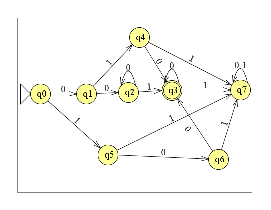
\includegraphics[width=0.8\columnwidth]{chap3/Imagenes/GrafoDirigido.eps}
\caption{Ejemplo de un grafo dirigido.}
\label{fig:igrafoD}
\end{figure}


\subsection{Teor\'ia de \'arboles}
En t\'erminos matem\'aticos un \'arbol es un grafo $T$ el cual se puede definir de
 la siguiente forma\cite{SUSANNAS.EPP2012}:

\begin{itemize}
	\item ``Un grafo se llama \'arbol si y solo si, est\'a libre de circuitos y
	 es conexo.''
	\item ``Un v\'ertice de grado 1 en $T$ se denomina un v\'ertice terminal (o
	 una hoja).''
	\item ``Un v\'ertice de grado superior a 1 en $T$ es un v\'ertice interno (o
	 un v\'ertice de rama).''
\end{itemize}


Los \'arboles son muy usados en la actualidad ya que permiten  darle sentido a
 la informaci\'on contenida, gracias a la asociatividad, parentizaci\'on y
 prioridad que este permite de manera impl\'icita. Entre sus usos m\'ultiples en
 el \'area de la inform\'atica se pueden destacar los  siguientes; relaciones
 entre m\'odulos de programaci\'on, \'arboles de decisi\'on en inteligencia artificial
 y representaciones gram\'aticas\cite{gutierrez1999estructuras}.  

Una forma de ver a un \'arbol puede ser como un solo nodo, est\'e recibe el nombre
 de  nodo ra\'iz, al cual se le puede enraizar un sinf\'in de \'arboles lo que da
 origen  a un \'arbol con otras caracter\'isticas, dependiendo del resultado se le
 puede clasificar en alguno de los modelos existentes, por ejemplo; \'arbol 
 general o \'arbol binario\cite{gutierrez1999estructuras},el mostrado en la figura
 \ref{fig:iarbol}, es un \'arbol binario que representa la jerarqu\'ia e 
 interconexi\'on entre varios procesadores. 

\begin{figure}[h]
\centering
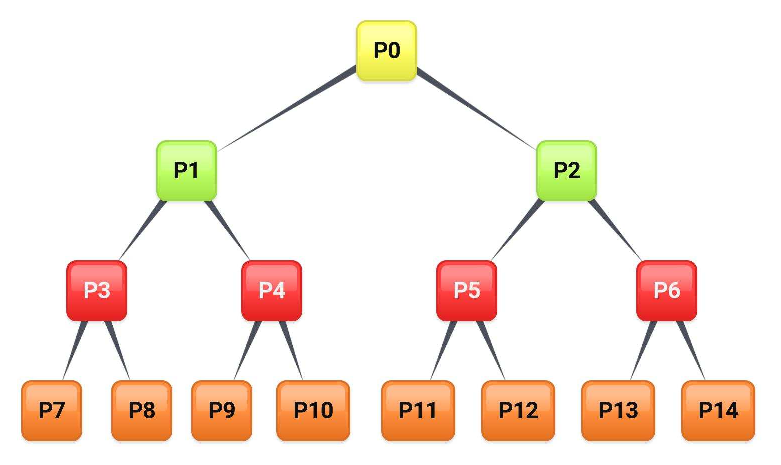
\includegraphics[width=0.8\columnwidth]{chap3/Imagenes/Arbol.eps}
\caption{Ejemplo de un \'arbol.}
\label{fig:iarbol}
\end{figure}

El \'arbol general es un modelo con una cantidad indeterminada de nodos hijos,
 mientras que el \'arbol binario es un caso particular del \'arbol general ya que
 este tiene la caracter\'istica de tener siempre en cada nodo 2 nodos hijos como
 m\'aximo, cabe mencionar que este es uno de los modelos a mas usados, as\'i como
 el ultimo caso mencionado, hay\'arboles que tienen una cantidad fija de nodos
 hijos, de manera general estos son llamados arboles n-arios
 \cite{gutierrez1999estructuras}.
\section{Tipos de datos}

En miner\'ia de datos existen 2 clasificaciones de datos\cite{Yang2010}, los cualitativos(por ejemplo: tipo de sangre, opini\'on personal, c\'odigo postal, tel\'efono) y num\'ericos. A continuaci\'on se presentan sus caracter\'isticas.

\begin{itemize}
\item Cualitativos o categ\'oricos\cite{Yang2010} 
	\begin{itemize}
	\item Son lo que se pueden ubicar en distintas  categor\'ias.
	\item Algunos se pueden ordenar en orden significativo
	\item No se le puede aplicar operaciones matem\'aticas
	\end{itemize}
	 

\item Cuantitativos\cite{Yang2010}
	\begin{itemize}
	\item Son de naturaleza num\'erica. 
	\item Se pueden clasificar en orden. 
	\item Admiten operaciones aritm\'eticas significativas. 
	\item Pueden ser discretos o continuos.		
	\end{itemize}
\end{itemize}

Los datos tambi\'en se pueden clasificar por la forma en que se categorizan, cuentan o miden. Este tipo de clasificaci\'on utiliza escalas de medici\'on, y cuatro niveles comunes de escalas son: 

\begin{itemize}
\item Nominal\cite{Yang2010}:
	\begin{itemize}
	\item Se clasifican los datos en categor\'ias mutuamente excluyentes (no superpuestas) y exhaustivas en las que no se puede imponer un orden o clasificaci\'on significativa en los datos. 
	\end{itemize}
		
\item Ordinal\cite{Yang2010}:
	\begin{itemize}
	\item Se clasifican los datos en categor\'ias que se pueden clasificar. 
	\item Las diferencias entre los rangos no pueden calcularse mediante aritm\'etica.
	\item Se pueden ordenar
	\end{itemize}		

\item Intervalo\cite{Yang2010}: 
	\begin{itemize}
	\item Se clasifican los datos y las diferencias entre las unidades de medida se pueden calcular mediante aritm\'etica. 
	\item El cero en el nivel de intervalo de medici\'on no significa \emph{null} o \emph{nada} como cero en aritm\'etica.
	\end{itemize}		

\item Relaci\'on\cite{Yang2010}:
	\begin{itemize}
	\item Se clasifican los datos y las diferencias entre las unidades de medida se pueden calcular mediante aritm\'etica. 
	\item El cero en el nivel de intervalo de medici\'on significa \emph{null} o \emph{nada} como cero en aritm\'etica.
	\end{itemize}
		
\end{itemize}


En este cap\'itulo se present\'o un breve marco de lo que es el aprendizaje
 m\'aquina y la teor\'ia necesaria para el desarrollo de un software capaz de 
 identificar secuencias de acciones a partir de una lista de acciones, en 
 resumen, se desarrollar\'a un sistema, con el paradigma de la POO, que genere 
 un grafo dirigido y en cada v\'ertice se almacenara la informaci\'on de cada 
 elemento de la lista de acciones consider\'andolo como un dato nominal, es 
 decir, un dato que carece de orden o valor inherente, dado que no hay
 relaci\'on num\'erica o de precedencia entre los datos, por lo que, con lo 
 \'unico que se puede trabajar es el orden de aparici\'on, relaci\'on 
 representada por el grafo dirigido, adem\'as el uso de un contador de 
 incidencias en cada v\'ertice. De este modo es posible identificar el camino 
 con los v\'ertices m\'as usados, esto es, las secuencias que se han repetido 
 mas veces, lo cual es el objetivo de esta tesis.
